\section{Convolutional Neural Networks}\label{sec:cnn}

Convolutional Neural Networks, and deep CNNs in particular, proved to be very effective in image classification tasks, as shown in the \textit{ImageNet Large Scale Visual Recognition Challenge} (see figure \ref{fig:cnn1}). By the way, this model is used also for semantic segmentation, detection, interpretation of pose and actions, even within videos (spatial and temporal streams).

\begin{figure}[h!]
    \centering
    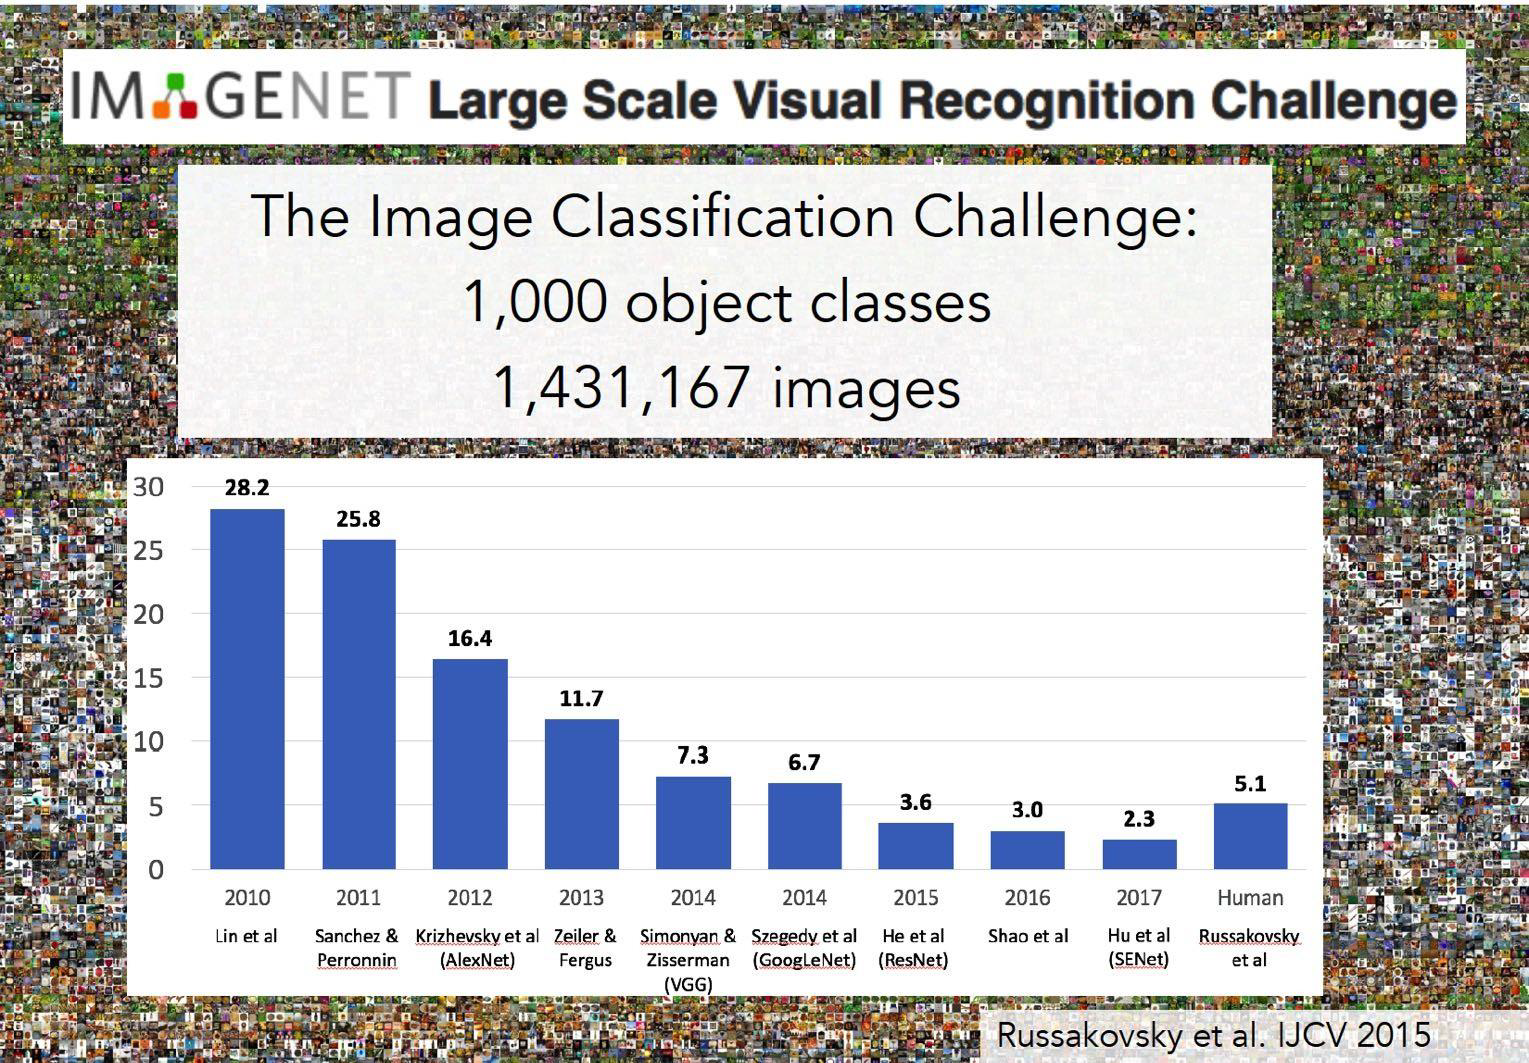
\includegraphics[width=0.7\linewidth]{cnn1}
    \caption[Successes of Deep CNNs]{Successes of Deep CNNs}
    \label{fig:cnn1}
\end{figure}

As we saw in section \ref{sec:dl-nn}, in a \textbf{traditional NN} with an input of size $N$ and a hidden layer of size $M$
\begin{myitem}
    \item the weight matrix $W$ has size $N \times M$,
    \item each node of the hidden layer is connected to each node of the input layer (that's why it's called \textit{fully connected NN}),
    \item it can be seen as with $M$ ``kernels'' which have dimension $N$ each,
    \item there are many parameters, thus it suffers severe overfitting.
\end{myitem}
Since spatial correlation is local, and it is what mostly interests in image-related tasks, we can reduce the number of parameters per layer, to put resources elsewhere. By applying this principle, we obtain a \textbf{locally connected NN}:
\begin{myitem}
    \item the output is based only on the \textit{receptive field} of size $P<N$, so $W$ is $P \times M$,
    \item now we have only $M$ kernels each with dimension $P$,
    \item there are less parameters to train, so less overfitting,
    \item this approach is meaningful since image data are stationary: statistics is similar at different locations.
\end{myitem}
The next step is to share the same parameters across different locations:
\begin{myitem}
    \item apply convolution with learned kernels,
    \item $W$ has size $P \times 1$,
    \item even fewer parameters to train,
    \item can simultaneously train many maps to extract more features (learns multiple filters).
\end{myitem}

This approach is particularly useful for images: while standard NNs scale quadratically with the size of the input and don't leverage stationarity, \textbf{Convolutional NN} connect each hidden unit to a small patch of the input and share the weight across hidden units.\\
By \textit{pooling} filter responses at different locations, we gain robustness to the exact spatial location of features.


\subsection{The architecture of CNNs}\label{sec:cnn-architecture}

Characteristics of CNNs:
\begin{myitem}
    \item Feed-forward:
    \begin{itemize}
        \item convolve input,
        \item non-linearity (rectified linear),
        \item pooling (subsampling - see later);
    \end{itemize}
    \item Supervised;
    \item Train convolutional filters by back-propagating classification error.
\end{myitem}

\begin{figure}[h!]
    \centering
    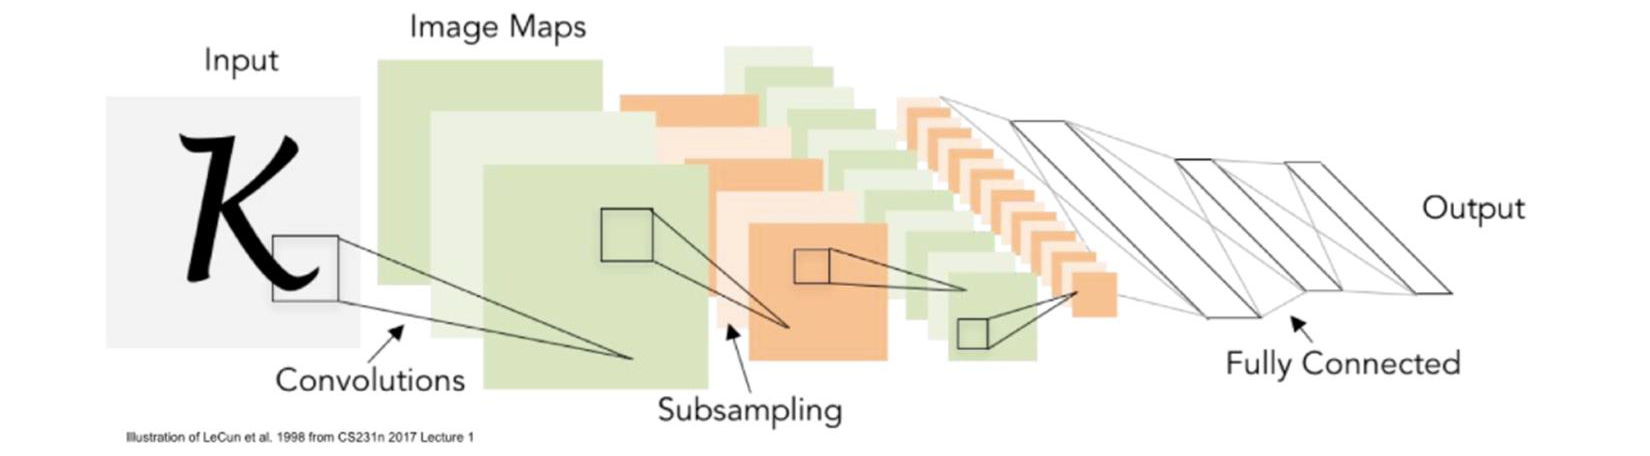
\includegraphics[width=\linewidth]{cnn2}
    \caption[Convolutional Neural Network]{Convolutional Neural Network}
    \label{fig:cnn2}
\end{figure}

Differently from a fully connected layer, a \textit{convolution layer} preserve the original spatial structure, by sliding over the image spatially, computing dot products. The matrix resulting from the application of each filter is called \textit{activation map}. Each filter produces higher level features, which at the last level compose a linearly separable classifier.\\
Note that filters always extend the full depth of the input volume.

The size of the produced activation map with respect to the input size depends on the filter size, and on the stride (how much to slide the filter over the input image). If the filter doesn't fit the image with the fixed stride, a zero-padding is applied.\\
Thus, a convolutional layer of size $W_1 \times H_1 \times D_1$ with $K$ filters of size $F$, stride $S$, amount of zero-padding $P$, produces a volume of size $W_2 \times H_2 \times K$, where
\begin{flalign}\label{eq:cnn-size-conv}
    &W_2 = \frac{W_1 - F + 2P}{S + 1},\\
    &H_2 = \frac{H_1 - F + 2P}{S + 1}.
\end{flalign}
The total number of parameters that have to be learned is $(F \cdot F \cdot D_1) \cdot K$ weights plus $K$ biases.

To go on with the brain-NN analogy, we can say that an activation map is a sheet of neuron outputs: each is connected to a small region in the input and all of them share parameters.

The \textit{pooling layer} makes the representations smaller and more manageable, and operates over each activation map independently. Possible pooling functions are max pooling or average pooling.\\
With an input of size $W_1 \times H_1 \times D_1$, size $F$ and stride $S$, it produces a volume of size $W_2 \times H_2 \times D_1$, where
\begin{flalign}\label{eq:cnn-size-pool}
    &W_2 = \frac{W_1 - F}{S + 1},\\
    &H_2 = \frac{H_1 - F}{S + 1}.
\end{flalign}


Usually, many layers with small filters are used, since smaller filters are easier to learn. Moreover, the depth of a network is very important, since reducing it the performance drops.

Another important aspect that needs to be underlined, is the invariance property: CNN are invariant with respect to translation, scale, rotation.


\subsection{Visualizing CNNs}\label{sec:cnn-visualize}

Raw coefficients of learned filters in higher layers are difficult to interpret.

Several approaches look to optimize input to maximize activity in a high level feature.

A common approach to map activations at high layers back to the input is to use \textbf{Deconvolutional Networks}:
\begin{myitem}
    \item They apply the same operations as CNNs, but in reverse: unpool feature maps, then convolve unpooled maps;
    \item In this case they are used as a probe, without inference or learning, as originally purposed;
    \item The result is a set of portions of an input image that give strong activation of the given feature map, which gives a non-parametric view on invariances learned by the model;
    \item From this, you can retrieve patches of validation images that give maximal activation of a given feature map.
\end{myitem}
